\subsection{Metrics}\label{sec:metrics}
Performance metrics are indispensable for evaluating the efficacy of outlier detection algorithms and facilitating rigorous comparative analyses between disparate methodologies.
Selecting appropriate metrics is a complex yet critical endeavor to ensure that empirical findings remain robust and interpretable.
This selection process necessitates a balance between two primary requirements: 
The utilization of metrics widely established within the scientific community to maintain benchmarking standards, and the adoption of metrics specifically suited to the inherent challenges of outlier detection, such as extreme class imbalance. 
Failure to align metric selection with the specific \todo{dataset specific?} properties of the dataset and the research objectives may lead to misleading conclusions regarding a model's predictive performance. \todo{source}



An analysis of 276 publications documenting model performance identifies the True Positive Rate ($TPR$), also referred to as sensitivity, recall, or the detection rate \todo{source},as the most frequently utilized metric. 
This is frequently supplemented by the False Positive Rate ($FPR$), or false alarm rate, which was reported in 116 of the surveyed papers and quantifies the frequency with which benign instances are erroneously classified as anomalies. 
A significant finding of this literature review is that 64 out of 290 papers relied exclusively on a single metric, typically Accuracy or the Area Under the Receiver Operating Characteristic Curve ($AUC$). 
Such a reductive evaluation is often insufficient for a comprehensive assessment of qualitative performance, especially in datasets characterized by extreme class imbalance. \todo{even AUC?}
In addition to predictive accuracy, a subset of the literature incorporates computational performance indicators, such as CPU utilization, execution time, and specific training or testing durations. 
These metrics are essential for evaluating the operational efficiency and scalability of an algorithm. \todo{maybe explain here why I dont use it}
These findings corroborate the research by \citep[postfix]{nassif2021}, which highlights the ubiquity of TPR while noting that FPR was reported in only a minority of the surveyed studies, alongside a secondary focus on various measures of computational latency.


The confusion matrix serves as the fundamental basis for deriving various scientifically accepted performance metrics, see figure \ref{fig:confusionmatrix}. \todo{source}
While certain basic metrics are less frequently applied in the specific context of outlier detection due to class imbalance, they remain widely recognized within the broader research community and provide the necessary context for more complex evaluations.


Consequently, this section first addresses fundamental metrics before proceeding to the $Accuracy$, $Precision$, $Specificity$ and $F1-score$,. 
After that I will covers threshold-agnostic metrics, specifically the Area Under the Receiver Operating Characteristic Curve ($AUC-ROC$) and the Area Under the Precision-Recall Curve ($AUC-PRC$).
Finally, I will argue, which metric I will use in my experiments.


\subsubsection*{Confusion Matrix}
In the context of outlier detection, which is framed as an imbalanced binary classification problem, performance is evaluated using a $2\times2$ confusion matrix. 
This matrix facilitates a direct comparison between the predicted classifications and the actual ground truth labels. 
The structure of the confusion matrix is organized such that the horizontal axis represents the predicted classes generated by the detection method, while the vertical axis represents the true classes. 
Each observation is assigned to one of the four cells based on this comparison: True Positives ($TP$) and True Negatives ($TN$) represent correct identifications of anomalies and inliers, respectively, whereas False Positives ($FP$) and False Negatives ($FN$) represent misclassification errors. 
This systematic categorization serves as the empirical foundation for calculating more complex performance metrics that account for the specific requirements of anomaly detection.


\begin{figure}[h] 
    \centering
    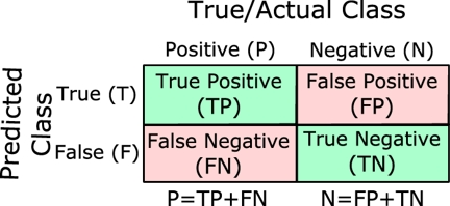
\includegraphics[width=0.6\linewidth]{Images/Confusion_Matrix.pdf}
    \caption{Confusion Matrix}
    \label{fig:confusionmatrix}
\end{figure}


In scientific literature, a heuristic \todo{wording what do I mean?} approach is frequently adopted to address the classification of instances. 
A significant disadvantage of these methods is the requirement for a predetermined threshold to distinguish outliers from inliers. \todo{why?} \todo{source}
In practical applications, the exact outlier ratio is typically unknown and must be estimated from historical data. \todo{source}
The selection of this threshold involves a critical trade-off: a threshold that is too high increases the number of false negatives, while a threshold that is too low elevates the number of false positives. 
The implications of these errors vary significantly depending on the application domain and may result in suboptimal decision-making. 
Within the context of Outlier Detection research, where benchmark datasets are available, the known outlier ratio is often utilized as the threshold to prevent the selection of arbitrary values. \todo{source} \todo{why?}
This standardization ensures a consistent framework for the comparative evaluation of different outlier detection methodologies. 
The most prevalent metrics derived from the confusion matrix include:


Accuracy is formally defined as:
\begin{equation}
        \text{Accuracy} = \frac{TP + TN}{TP + FN + FP + TN}.
\end{equation}

It measures the overall effectiveness of a method by calculating the proportion of correctly classified instances relative to the total number of observations. \todo{source}
Its main advantage is its intuitive interpretability and its inclusion of all classes.  
A primary disadvantage of this metric is that it can be misleading in the presence of significant class imbalance, particularly when a method fails to identify any instances as outliers. 
The model may achieve a high accuracy score simply by classifying all instances as inliers, thereby ignoring the minority class entirely. 
This results in a performance measure that does not accurately reflect the model's ability to detect anomalies. \todo{add pros}


Precision is formally defined as:
\begin{equation}
        \text{Precision} = \frac{TP}{TP + FP}
\end{equation}

Precision quantifies the proportion of correctly identified anomalies relative to the total number of instances classified as positive, encompassing both true positives and false positives. \todo{source}
This metric emphasizes the degree of agreement \todo{define} between the ground truth labels and the positive predictions generated by the classifier. 
A notable disadvantage of prioritizing precision is that it may encourage conservative classification behavior as well, as a model might optimize its score by identifying only the most conspicuous outliers. 
Any false positive increases the denominator of the precision formula, thereby reducing the overall score. 
Furthermore, this metric fails to account for false negatives, which tend to increase when a model adopts a conservative threshold. 
Such a limitation is particularly problematic in high-stakes scenarios, such as fraud detection or medical diagnosis, where the costs associated with failing to identify an anomaly are substantial. \todo{source or heuristic}


Recall is formally defined as:
\begin{equation}
        \text{Recall} = \frac{TP}{TP + FN}
\end{equation}

Recall, also referred to as True Positive Rate or sensitivity, measures the proportion of correctly identified outliers relative to the total number of actual anomalies in the dataset. \todo{source}
This metric effectively evaluates the model's ability to capture the entire anomaly class. 
A significant disadvantage of prioritizing recall is that it can incentivize a high number of false positives, as a model can maximize its score by indiscriminately classifying a large portion of the dataset as anomalous.
While the denominator remains constant regardless of the number of false positives, the focus on maximizing the numerator (true positives) often leads to a lower classification threshold \todo{bt threshold is set by me}.
This is particularly problematic in industrial contexts, such as manufacturing, where a detected outlier might trigger an emergency shutdown.
In such cases, frequent false alarms result in substantial operational costs and unnecessary downtime. \todo{sournce or heuristic} 


Specificity is formally defined as:
\begin{equation}
        \text{Specificity} = \frac{TN}{FP + TN}
\end{equation}
Specificity, also known as the True Negative Rate ($TNR$), quantifies the proportion of correctly identified inliers relative to the total number of actual negative instances in the dataset. 
This metric focuses exclusively on the negative class, serving to evaluate the effectiveness of a method in correctly rejecting non-anomalous observations. 
In the context of outlier detection, high specificity indicates that the model is proficient at avoiding false alarms, thereby ensuring that normal instances are not misclassified as anomalies. \todo{pros and cons}


\todo{transition, write about metrics with an inverse relationship}
It exists an inherent inverse relationsip between precision and recall. 
Balancing these two metrics is essential for an objective evaluation of outlier detection performance, especially within imbalanced data structures. 
This interdependency forms the basis for more complex evaluations, such as $F1-Score$, Area under the Recever Operator Charakteristics ($AUC-ROC$) and Area Under the Precision-Recall Curve ($AUPRC$). 


The $F1-score$ represents the harmonic mean of precision and recall, providing a unified metric that accounts for the bevormentioned inverse relationship. 
It is formally defined as the harmonic mean:

\begin{equation}
    F_1 = 2 \cdot \frac{\text{Precision} \cdot \text{Recall}}{\text{Precision} + \text{Recall}}
\end{equation}

The score is significantly influenced by the lower value of the two values.
If either precision or recall is low, the F1-score will be lower than a simple arithmetic mean would suggest. 
Consequently, a high $F1-score$ is only achievable when both precision and recall are simultaneously high. 
Adjustments to the classification threshold increases typically one result and decreases the other. 
By optimizing the $F1-score$, the model effectively seeks a balance that minimizes both false positives and false negatives, making it a robust evaluation tool for imbalanced outlier detection tasks. 
The $F1-score$ is threshold-dependent. 
Consequently, any modification to this threshold directly influences the resulting $F1-score$. 


A primary critique of the $F1-score$ is its exclusion of correctly identified inliers, or true negatives. 
In the field of outlier detection, where the inlier class constitutes the vast majority of the observations, a metric that disregards the model's proficiency in identifying the normal class provides a technically incomplete assessment of overall performance.
Furthermore, the $F1-score$ assigns equal weight to precision and recall. 
In many practical applications, an equal trade-off may not align with the specific cost-benefit requirements of the domain. 
For instance, in a medical context, diagnosing a healthy patient with a condition may be considered less severe than failing to detect a life-threatening illness. 
Similarly, in a legal or security context, misclassifying an individual as high-risk could lead to disproportionately severe consequences. 
Depending on the specific domain of the analysis, this can be addressed by reweighting the importance of recall or precision. 
This leads to the $F_\beta$ family of metrics, such as the $F2-score$, which prioritizes recall, or the $F0.5-score$, which places greater emphasis on precision. \todo{why dont I use these? I already performed data analysis} 
\todo{conclusion why do I use F1 and not the others?}


\subsubsection*{Agnostic Metrics}
To solve the disadvantages of threshold-depended metrics, threshold-agnostic metrics are frequently employed in the scientific community. 
$ROC AUC$ and $AUPRC$ are most prominent metrics frequently employed. 
These metrics evaluate the performance of a model across all possible threshold values, providing a more comprehensive assessment of its discriminative capability.
Due to its extensive application in cost-benefit decision analysis, both the $ROC AUC$ and the $AUPRC$ are highly suitable for learning tasks characterized by asymmetric cost functions and imbalanced datasets.
For example, $ROC AUC$ is a metric used for effective assessment of intrusion detection systems \citep[postfix]{nassif2021}.

\todo{formally define}
$ROC AUC$ serves as an aggregate performance metric evaluating a model with values constrained between 0 and 1. 
Those values represents the probability that a randomly selected outlier receives a higher anomaly score than a randomly selected inlier.
Consequently, higher values indicate a superior capability of the model to distinguish between these two classes. 
As illustrated in the figure, the ROC curve plots the $Recall$ on the ordinate against $1-Specificity$, also known as $FPR$, on the abscissa.
The area under this curve is mathematically defined by the integral.


Visually, a higher ROC AUC corresponds to a curve that bends toward the coordinate (0,1), where $AUC=1$ signifies a perfect classification with minimal $FPR$ and maximal $TPR$. 
A value of $AUC=0.5$ indicates that the model's predictive performance is equivalent to random chance, which establishes a baseline for comparative analysis and is visually represented by a diagonal line. 
Conversely, $AUC=0$ indicates that the model perfectly misclassifies outliers as inliers and vice versa, resulting in a curve that bends toward the coordinate (1,0).

\todo{insert image}


The $ROC AUC$ offers distinct advantages for imbalanced datasets, yet it also presents significant limitations. 
In such contexts, $ROC AUC$ can yield overly optimistic assessments because its calculation incorporates the $FPR$. 
Since the number of true negative instances typically far exceeds the number of true positives, the denominator of the $FPR$ becomes dominated by true negatives \citep{davis2006relationship}. 
Consequently, the shift in the $FPR$ resulting from the misclassification of inliers remains marginal. 
In imbalanced datasets, the $FPR$ tends to remain low, which biases the curve toward the upper-left coordinate and may obscure poor model performance. 
A key strength of $ROC AUC$ is its consistency across varying outlier ratios, which facilitates reliable comparisons between different models.


The Area Under the Precision-Recall Curve (AUPRC) addresses the tendency of $ROC AUC$ to provide overly optimistic performance assessments by excluding true negatives from its calculation, thereby focusing on the primary objective of detecting true positive instances. 
Precision and recall exhibit a non-monotonic trade-off relationship; as one metric increases, the other typically decreases. \todo{is that whats in the diagram?}
This represents the inherent tension between identifying every outlier (recall) and ensuring those identified are correctly classified (precision). 


The $AUPRC$ is bounded between 0 and 1, where a value of 1 signifies a perfect model that correctly identifies all outliers without false positives. 
As illustrated in the figure, the $AUPRC$ plots recall on the abscissa against precision on the ordinate, with superior model performance indicated by a curve that extends toward the upper-right coordinate. 
It is formally defined as the integral of the precision-recall curve, which is calculated by varying the classification threshold across its entire range.
\todo{define it properly} 


The curve generally declines as the classification threshold is lowered and outliers are ranked. 
At strict thresholds, only the most definitive outliers are identified, resulting in high precision but low recall. 
Conversely, lowering the threshold increases recall but also the likelihood of misclassification, which reduces precision and causes the curve to trend toward the lower-right region of the diagram.
\todo{insert citation etc, see davis2006relationship}
\todo{insert paper saito2015precision, difference between ROC and AUPRC}


Unlike the $ROC AUC$, the $AUPRC$ does not possess a fixed baseline.
Instead, the baseline is determined by the specific dataset and corresponds to the outlier ratio. 
In the case of a naive model with no discriminative power, the model effectively guesses the outlier status by varying its threshold.
The probability of such a model identifying a true positive is equal to the prevalence of outliers within the dataset. 
As the classification threshold becomes more lenient, the model identifies a greater number of true positives, thereby increasing recall. 


However, precision remains constant because the proportion of outliers is fixed.
The increase in true positives occurs proportionally to the increase in false positives. 
Consequently, the baseline for a non-discriminative model is represented by a horizontal line at the level of the outlier ratio. 
This framework allows for the performance comparison of different methods in a given dataset: if the curve of Model A consistently remains above that of Model B, Model A demonstrates superior performance. 
If the curves intersect, one model may be better suited for tasks requiring high precision, while the other excels in high-recall applications. \todo{good in the results or disc}
If a model's curve coincides with the baseline, its performance is equivalent to random guessing. 


To summarize the advantages and disadvantages associated with the aforementioned metrics, preceding the selection and justification of the specific metric employed in this analysis. 
While Accuracy, Precision, Recall, and Specificity are derived from the fundamental components of the confusion matrix, these values are intrinsically dependent on the selected classification threshold.
In real-world applications, the optimal threshold is often unknown and must be estimated, which introduces a degree of subjectivity and potential bias into the evaluation process.


Accuracy remains a prevalent metric in the field, as discussed above.
However, Accuracy is fundamentally inadequate for outlier detection due to the inherent class imbalance of such datasets. 
The rest of the beforementioned metrics are class-specific metrics, resulting in an incomplete evaluation of model performance if a single one is chosen.


%Consequently, performance metrics for imbalanced datasets must account for the actual class distributions to ensure an objective evaluation \citep[p.8]{branco2016survey}.
The F1-score was selected as the primary evaluation metric because it harmonizes precision and recall, including information of all classes but the true negatives.
It offers a balanced assessment of model efficacy within the domain of outlier detection. 
While this metric does not account for true negatives, its application is justified by the characteristics of the Wine dataset, which represents a domain where the costs associated with false positives and false negatives are equivalent. 
Consequently, the $F_\beta$ family of metrics was bypassed, as those measures are designed to prioritize either precision or recall based on specific weighting. 
Furthermore, the inclusion of the F1-score is essential for the rigorous testing of the research hypothesis, as the previously documented performance of the k-nearest neighbors algorithm was established using this specific metric, necessitating a consistent basis for comparison.


The $AUC ROC$ and $AUPRC$ will be incorporated into the analysis to provide a comprehensive evaluation of model performance. 
The $AUC ROC$ evaluates the efficacy of prediction ranking rather than absolute classification values, establishing a robust baseline against a random classifier that facilitates standardized comparisons. 
In contrast, the $AUPRC$ provides a more nuanced interpretation of the outlier class by concentrating on the successful detection of anomalies while minimizing the incidence of false positives. 
This metric is particularly informative in the context of imbalanced datasets, as it prioritizes the precision-recall trade-off inherent in identifying rare instances. 
Collectively, these metrics ensure that both the general discriminative power and the specific accuracy regarding the minority class are rigorously quantified.











